% ---------------------------------------------------------------------------- %
\section{Linguometer data collection}
\label{ch:experiments}
% ---------------------------------------------------------------------------- %
In order to determine whether knowledge of motor activity during speech
can aid learning to perceive speech, a constellation of instruments and
software has been used to measure speech-related phonoarticulatory activity.
The novel setup, informally called
the Linguometer, was realized for characterizing 
the motor processes of speech production by the simultaneous acquisition of data
during articulation in many modalities: ultrasound, articulograph,
laryngograph, and audio-video recording. 
The short term goal is to identify motoric invariants that share a common 
structure during the production of speech.
Moreover, the acquired data will be used to train a Bayesian speech recognizer
based on the motoric representation of speech (Section~\ref{ch:linguometer:instrumentation}).

\begin{table}[ht!]
  \begin{center}
  \begin{scriptsize}
	\begin{tabular}{|c|c|c|}
	  \hline
	  \textbf{Exp./Subj.} & \textbf{Gender} & \textbf{Age}\\
	  \hline
	  1 & Female & 23\\
	  2 & Female & 30\\
	  3 & Female & 23\\
	  4 & Female & 21\\
	  5 & Female & 25\\
	  6 & Female & 24\\
	  7 & Male & 25\\
	  8 & Male & 26\\
	  9 & Male & 26\\
	  \hline
  \end{tabular}
  \end{scriptsize}
  \end{center}
	\caption[Subjects' age and gender]{\textbf{Subjects' age and gender}: 
	a total of nine subjects have been recorded by means of the Linguometer.
	Despite the fact that male subjects are generally more complicated to record
	than female ones, three males have been recorded.}
 \label{tab:experiments:subjects}
\end{table}

The Linguometer setup has been used to acquire data produced by Italian
speakers. 
Nine speakers of Lecce Italian were asked to read three times a corpus of words
and pseudo-words (Table~\ref{tab:experiments:subjects}).
Both words and pseudo-words were chosen in order to include all consonantal and
vocalic phonemes present in Italian. 
Words were mainly stress-initial, with target consonants in word initial 
position, followed by /a, e, i, o, u/ vowels. 
Some instances of words with different stress position were also included.
Speakers read the word set three times with declarative intonation and three 
times with interrogative intonation. 
The pseudo-word set was composed by a sequence of monosyllables, where all 
consonantal phonemes of Italian were included, followed by /a, u, i/ vowels. 
The goal of this Section is to introduce the reader to the experimental protocol
followed during the nine Linguometer investigations.
% ---------------------------------------------------------------------------- %
\subsection{Experimental protocol}
\label{sec:experiments:protocol}
% ---------------------------------------------------------------------------- %
The Linguometer setup has been used to collect a large and consistent dataset
of phono-articulatory features.
The CRIL laboratory\footnote{Prof. M. Grimaldi, Dr. B. Gili Fivela} selected a
total of 74 words and 68 pseudo-words (monosyllables) suitable for the 
investigations.
Similarly to the Mirror Project~\citep{metta.etal:2006}, the data acquired
with the Linguometer will be
used to investigate to what extent the system could learn invariances across 
different gestures, in this case the gestures of speech, relying on motor 
information for classification.
Furthermore, it is needed to test the Bayesian model in different contexts as 
\citet{metta.etal:2006} have done recording the grasping actions from several
different viewpoints (Section~\ref{ch:linguometer:instrumentation}).
For those reasons, the 74 words have been submitted in two different
phonetical contexts such as declarative and interrogative intonations.
\begin{table}[htbp]
  \begin{center}
  \begin{scriptsize}
	\begin{tabular}{ccccc}
	  \hline
	  accento & \`ancora & ancora & ancoraggio & bacco\\
	  baffo & biro & birra & bronzo & bruchi\\
	  buchi & buco & bucone & bufalo & buffo\\ 
	  calza & carretto & carro & cefalo & ceffo\\
	  cero & cirro & faro & farro & fascia\\
	  fasciatoio & fazzoletto & gelato & gelo & ghiro\\
	  giallo & goffo & gozzo & gru & gufo\\
	  lava & lavatoio & legnaia & legno & mamma\\
	  matto & mattone & mirra & mito & moro\\
	  muffa & nome & none & nonne & nonnetto\\
	  notaio & papa & papa & pappa & pelato\\
	  pozzo & psicologo & scaglione & scempia & scoglio\\
	  semi & semola & sera & serra & sommi\\
	  strada & terra & toro & tuffo & tufo\\
	  uovo & vaso & vassoio & yogurt & \\
	  \hline
  \end{tabular}
  \end{scriptsize}
  \end{center}
	\caption[Corpus - words (declarative intonation)]{\textbf{Corpus - words
	(declarative intonation)}: the subjects were asked to read three times 
	74 declarative words.}
 \label {tab:experiments:stimuli:wa}
\end{table}



\begin{table}[htbp]
  \begin{center}
  \begin{scriptsize}
	\begin{tabular}{ccccc}
	  \hline
	  accento?  & \`ancora?  & ancora?  & ancoraggio?  & bacco?\\
	  baffo?  & biro?  & birra?  & bronzo?  & bruchi?\\
	  buchi?  & buco?  & bucone?  & bufalo?  & buffo?\\ 
	  calza?  & carretto?  & carro?  & cefalo?  & ceffo?\\
	  cero?  & cirro?  & faro?  & farro?  & fascia\\
	  fasciatoio?  & fazzoletto?  & gelato?  & gelo?  & ghiro?\\
	  giallo?  & goffo?  & gozzo?  & gru?  & gufo\\
	  lava?  & lavatoio?  & legnaia?  & legno?  & mamma?\\
	  matto?  & mattone?  & mirra?  & mito?  & moro?\\
	  muffa?  & nome?  & none?  & nonne?  & nonnetto?\\
	  notaio?  & papa?  & papa?  & pappa?  & pelato?\\
	  pozzo?  & psicologo?  & scaglione?  & scempia?  & scoglio?\\
	  semi?  & semola?  & sera?  & serra?  & sommi?\\
	  strada?  & terra?  & toro?  & tuffo?  & tufo?\\
	  uovo?  & vaso?  & vassoio?  & yogurt?  & \\
	  \hline
  \end{tabular}
  \end{scriptsize}
  \end{center}
	\caption[Corpus - words (interrogative intonation)]{\textbf{Corpus - words
	(interrogative intonation)}: the subjects were asked to read three times 
	74 interrogative words.}
 \label {tab:experiments:stimuli:wi}
\end{table}




To sum up, three classes of stimuli have been submitted to the subjects 
during the investigations: 74 words both in the declarative and interrogative 
forms (e.g.: /ancora/, /mattone/ and /ancora?/, /mattone?/) and 68 syllables, 
for a total of 216 unique stimuli.
Moreover, each class of stimuli was submitted three times, for a grand total 
of 648 between words and pseudo-words recorded during each experiment.
The complete set of stimuli was recorded from nine subjects (six females and
three males, age 23-30) born nearby the city of Lecce and speaking Lecce
Italian.
As already discussed in Section~\ref{sec:linguometer:instrumentation:us}, it is to
some extent easier to record female subjects, due the smaller anatomical size of
the larynx.
Tables~\ref{tab:experiments:stimuli:wa}, \ref{tab:experiments:stimuli:wi} 
and~\ref{tab:experiments:stimuli:ss} show the stimuli used for the
Linguometer experiments while Table~\ref{tab:experiments:subjects} illustrates 
the age and the gender of the nine subjects.

\begin{table}[htbp]
  \begin{center}
  \begin{scriptsize}
	\begin{tabular}{ccccc}
	  \hline
	  asa & ba & cia & da & fa\\
	  ga & gia & glia & gna & ja\\
	  ka & la & ma & na & pa\\
	  ra & sa & scia & ta & va\\
	  wa & za$^a$ & za$^b$ & &\\
	  \hline
	  asu & bu & ciu & fu & giu\\
	  gliu & gnu & gu & ju & ku\\
	  lu & mu & nu & pu & ru\\
	  sciu & su & tu & vu & wu\\
	  zu$^a$ & zu$^b$ & &\\
	  \hline
	  asi & bi & ci & di & fi\\
	  ghi & gi & gli & gni & ji\\
	  ki & li & mi & ni & pi\\
	  ri & sci &  si & ti & vi\\ 
	  wi & zi$^a$ & zi$^b$ & &\\
	  \hline
  \end{tabular}
  \end{scriptsize}
  \end{center}
	\caption[Corpus - pseudo-words]{\textbf{Corpus - pseudo-words}:
	the subjects were asked to read three times 68 pseudo-words (syllables).
	Note: $^a$: /dz/; $^b$: /ts/.}
 \label{tab:experiments:stimuli:ss}
\end{table}


% ---------------------------------------------------------------------------- %
\subsection{Preparation of subjects}
\label{sec:experiments:preparation}
% ---------------------------------------------------------------------------- %
An investigation performed with the Linguometer required the subjects to come
over the CRIL laboratory twice.
Under normal conditions, one experiment required two days of work, the first
one for calibration and the second one for data recording.
In the first day, the subjects were asked to sit on the Linguometer stool. 
The height of the stool was then regulated so that the subjects' mouth was
perfectly inside the articulograph recording volume
(Section~\ref{sec:linguometer:instrumentation:ag}).
When the stool was appropriately regulated in height, the transducer stand was
calibrated both in depth and inclination. 
Adjusting the inclination of the stand usually requires calibrating its height as
well, using the wooden boxes described
in Section~\ref{ch:linguometer:instrumentation:custom}.

% ---------------------------------------------------------------------------- %
\begin{figure}
	\centering
	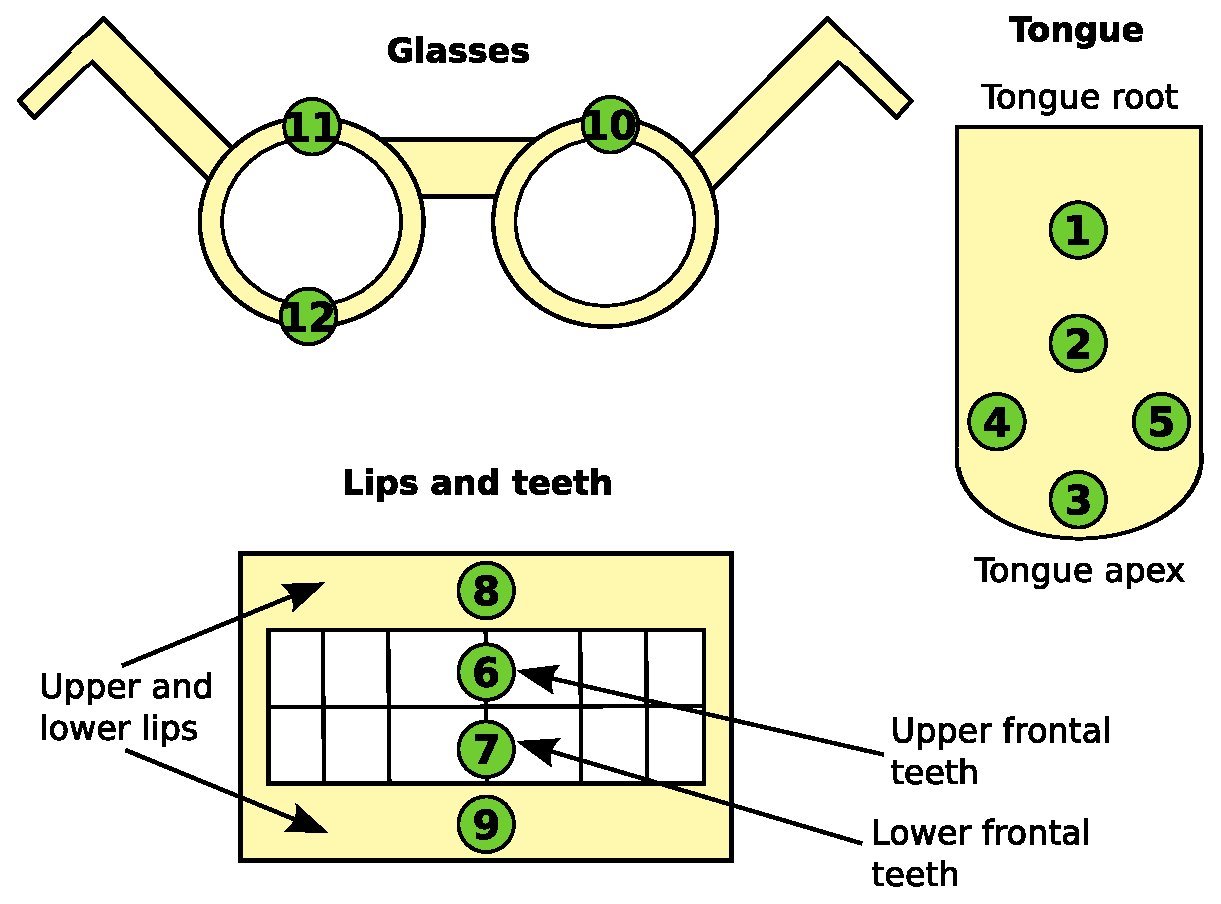
\epsfig{file=include/experiments/images/map.eps, width=0.75\textwidth}
	\caption[Sensor map]{\textbf{Sensor map}:
	in order not to stress the subjects, the experiments never took pictures 
	of the inaccessible sensors. For this reason, the sensor map provides a
	useful representation of the positions of the twelve sensors during
	the Linguometer recordings.
	Note: coronal view of the mouth (\emph{Lips and teeth}) and of the
	\emph{Glasses}; axial view of the \emph{tongue}.}
	\label{fig:experiments:map}
\end{figure}
% ---------------------------------------------------------------------------- %

The task of regulating the subjects' posture inside the Linguometer has to meet
two criteria. Firstly, the subject does need to feel as comfortable as possible,
in order not to alter the physiological mechanism of speech production.
%in order not to move during the recordings 
Lastly, the whole surface of the tongue must be visible in the ultrasonographic
reconstruction~(Section~\ref{ch:linguometer:instrumentation:custom}).
In fact, depending on the subject's anatomical properties, the ultrasonographic
transducer needs to be placed in a proper inclination in order to acquire
the complete surface of the tongue.
For those two reasons, the subject was asked to speak freely or to repeat
particular words that recruited important tongue movements
(e.g.: /birra/ and /carro/) so that the experimenters had the chance to verify
if the subject's posture was suitable both for the experimental requirements 
and for the subject's comfort.
The whole subject positioning procedure did not last more than half an hour. 

The adjustment of the position of the ultrasonographic transducer inside the
AG500 EMA-Cube involves moving the ultrasound transducer itself.
As explained in Section~\ref{sec:linguometer:instrumentation:ag}, the electromagnetic
interference caused by the presence of the transducer inside the recording area
of the articulograph can be compensated for by means of calibration.
For this reason, a complete calibration of the articulograph followed each
 adjustment of the subject's position.\\

% ---------------------------------------------------------------------------- %
\begin{figure}
	\centering
	  \subfigure[\label{fig:experiments:glue:1}]
		{\includegraphics[width=0.45\textwidth]{include/experiments/images/glue_1.tps}}
		\hspace{0.05\textwidth}
	  \subfigure[\label{fig:experiments:glue:2}]
		{\includegraphics[width=0.45\textwidth]{include/experiments/images/glue_2.tps}}

	\caption[Sensors gluing]{\textbf{Sensors gluing}:
	(a) a couple of film-coated AG500 sensors is shown (the film adheres
	perfectly onto the sensor). (b) Dr. Marisa Ferro is verifying if the sensors
	are properly glued onto the tongue of a subject (Subject 2,
	Table~\ref{tab:experiments:subjects}).}
	\label{fig:experiments:glue}
\end{figure}
% ---------------------------------------------------------------------------- %

The day after calibration, the subject came over for the actual
experiment.
The recording itself lasts circa 35 minutes, but a larger amount of time is
required to prepare the subject for the experiment and to test the Linguometer
devices and connections.
Firstly the articulograph AG500 sensors are coated using a thin polymeric 
film, previously sterilized\footnote{Household plastic film. The piece used
to cover the sensor is 
circa $1\times1$ cm in size.}. Once the first coating layer is applied, the 
sensors are covered with the \emph{Plasty-late} biocompatible liquid moulding 
compound\footnote{Plasty-late by Firma Glorex, Rheinfelden Grobmattstr, 
Germany.}. The second skin is applied simply by dipping the sensor inside the
liquid compound.
The sensors are then glued on the subject's articulators using the
\emph{Histoacryl} skin adhesive\footnote{Histoacryl by BBraun, Milano, Italy}.
The sensor-gluing procedure suggested by Carstens Medizinelektronik GmbH does 
not envisage covering the sensors with the plastic film before 
applying the second protective polymeric layer.
The experimenters found that this simple precaution protects the sensors
from damage when the \emph{Plasty-late} skin is removed. Furthermore, the thin
plastic film layer allows the experimenters to model the glued interface,
thus ensuring better adhesion between the coated sensor and the articulators.
Once the sensors are properly coated, they are sterilized and then 
glued onto the articulators using dentist tools or more simply attached
to the glasses using adhesive tape.
Furthermore, the band that holds the laryngograph electrodes in close contact
with the larynx is tightened to the subject's neck
(Section~\ref{ch:linguometer:instrumentation:lg}).
% ---------------------------------------------------------------------------- %
\subsection{Recording data}
\label{sec:experiments:recording}
% ---------------------------------------------------------------------------- %
Although the Linguometer recording procedure has already been discussed in
Section~\ref{sec:linguometer:architecture:diagram} (while describing the 
workflow and the data-streams diagrams), a brief clarification is made in 
this Section. 
Figure~\ref{fig:linguometer:architecture:workflow} shows the relevant
diagrams. In that example, the 
experimenters were
assumed to be submitting a total of two words (\wf{Word 0} and \wf{Word 1}) 
belonging to a single sequence.
Real experiments consist in acquiring a total of 648 between words and
syllables, divided in nine sequences (three classes of stimuli and
three repetitions for each class).
Figure~\ref{fig:experiments:exp} shows two subjects being recorded by the
Linguometer.

Once the sensing devices are attached to the subject's articulators, neck and
glasses, the subject sits inside the Linguometer.
Usually, while one experimenter trains the subject and coats the sensors, the
other one tests the recording devices and the synchronization mechanism.
This subdivision of the tasks allows the experimenters to shorten the interval
between subject preparation and the beginning of the recording session.
The investigation lasts circa 35 minutes
for a total of 20 GB of acquired data.
% ---------------------------------------------------------------------------- %
\begin{figure}
	\centering
	  \subfigure[\label{fig:experiments:exp:2}]
		{\includegraphics[width=0.45\textwidth]{include/experiments/images/exp_2.tps}}
		\hspace{0.05\textwidth}
	  \subfigure[\label{fig:experiments:exp:1}]
		{\includegraphics[width=0.45\textwidth]{include/experiments/images/exp_1.tps}}

	\caption[Experiments]{\textbf{Experiment}:
	two subjects being recorded by the Linguometer.}
	\label{fig:experiments:exp}
\end{figure}
% ---------------------------------------------------------------------------- %

% ---------------------------------------------------------------------------- %
\subsection{Off-line acquisition: profile of the palate}
\label{sec:experiments:palate}
% ---------------------------------------------------------------------------- %
In Section~\ref{sec:linguometer:instrumentation:us} 
%
%and in 
%Section~\ref{sec:speech:language:mechanism} 
%
the author discussed the
importance of the palate in the articulatory mechanism and 
explained why recording the palate's profile during speech production using 
the ultrasonographic system is not possible.

In this context, the profile of the palate has been acquired off-line, 
meaning after each experiment. 
In fact, the transducer was removed from its stand and placed submentally to the
subjects. 
Moreover, the experimenters asked the subjects to keep a small volume of water
in their mouth and to bend their necks 45$^o$ with respect to the sagittal
plane.
After the subjects bent their necks, the experimenters were able to record both
the tongue and the palate profiles, taking advantage of the liquid medium.
Figure~\ref{fig:results:pal} shows a frame from a palate-recording sequence.
In the Figure here shown, the subject is moving its tongue freely. 
The experimenters asked the subjects to push their tongue tips to the
palate and follow its profile.
Furthermore, the subjects kept the tongue in resting position, so that the
profile of the palate could eventually be matched onto the tongue profiles
acquired with the ultrasound system during the experiments.
% ---------------------------------------------------------------------------- %
\begin{figure}
  \centering
	\subfigure[\label{fig:experiments:pal:1}]
	{\includegraphics[width=0.45\textwidth]{include/experiments/images/palat_1.tps}}
	\hspace{0.05\textwidth}
	\subfigure[\label{fig:experiments:pal:2}]
	{\includegraphics[width=0.45\textwidth]{include/experiments/images/palat_2.tps}}

	\caption[Profile of the palate]
	{\textbf{Profile of the palate}: the profile of the palate has been recorded
	off-line by asking the subjects to keep water in their mouths.
	Furthermore, the subjects bent their necks of 45$^o$ over the sagittal
	plane.
	(a) A frame from the ultrasound system showing the acquired profile of the
	palate. (b) Hand-traced contours of the tongue dorsum and the 
	profile of the palate. Note: the tongue is not in the resting position.}
	\label{fig:results:pal}
\end{figure}
% ---------------------------------------------------------------------------- %


% ---------------------------------------------------------------------------- %
